%   MSc Business Analytics Dissertation
%
%   Title:     Aaa Bbbbbbb Cccccccccc
%   Author(s): Xxxxxx Xxxxxxxxx and Yyy Yyyyyyyyy
%
%   Chapter 4: Methodology
%
%   Change Control:
%   When     Who   Ver  What
%   -------  ----  ---  --------------------------------------------------------------
%   11Feb11  AB    0.1  Begun 
%

\chapter{Methodology}\label{C.Methodology}

\section{Overview}\label{S.Ch4.opening}
To assist financial auditor or stakeholder at financial institutions and banks, and to identify such loan portfolio which may default in future based on the geospatial information and financial data. This research work followed the KDD process which involves characteristics variables selection, perform data restructuring, data transformation and data mining for the deployment of a predictive model using visual analytics tools such as Tableau, QlikView, etc.
\section{Software \& Tools Specifications}\label{ch4.2}

\textbf{Software \& Tools used:}

Following is the list of tools and softwares that has been used while working on this project:
\begin{description}
  \item[Data Processing:] MS Excel 2017 and Alteryx Desginer 11.0
  \item[Version Control:] Github (github.com)
  \item[Dashboard:] Tableau Professional 10.2 and R Stuio 1.0.36
  \item[Data Storage:] Github Pages (https://pages.github.com/) and Google Drive
\end{description}
\textbf{R Packages used:}
\begin{description}
  \item[Packages required Logisctic Regression Model:] Following packages used to building simple regression and logistic regression based model for predictig the good or bad loan portfolio: glm() with class set to "bionomial" for Logistic Regression and "log" for Poisson regression, ROSE, ROCR, Dplyr, maps, ggplot2
  \item[Decession Tree:] Following r-packages used for building a predictive model based on decision tree: caret, rpart, rattle, ROSE, ROCR, RColorBrewer, party, partykit
\end{description}
\textbf{R Shiny:} R Shiny packages for building interactive dashboards: leaflet, maps, ggmap, gridExtra, htmlwidgets, reshape2. To deploy predictive model on Tableau to build dyanmic and easy to user dashboard R Server used


One may replicate our work on his/her computer having minimum hardware specifications outlined here. This research work carried on following machines. 

% \usepackage{booktabs}
\begin{table}[!htb]
\centering
\caption{System configurations used to carry out this research}
\label{osc4}
\begin{tabular}{|p{3cm}|p{5cm}|p{5cm}|}
\toprule
\textbf{Specification}    & \textbf{System 1 - Lenovo Yoga 500}   & \textbf{System 2 - Dell Inspiron 15} \\ \midrule
\textbf{Operating System} & Windows 10 Professional               & Windows 7 Professional               \\
\textbf{Processor}        & Intel(R) Core(TM) i3-5005CU @ 2.00GHz & Intel(R) Core(TM) i3-3217U @ 1.80GHz \\
\textbf{RAM}              & 4.00 GB                               & 4.00 GB                              \\
\textbf{System Type}      & 64-bit OS, x64-Based Processor        & 32 -bit Operating System             \\ \bottomrule
\end{tabular}
\end{table}


\section{Data}\label{ch4.3}

\subsection{Overview}
One requires the accessibility to the right set of data, and information on which statistical and modelling techniques can be applied to start any data oriented research in analytics domain, KPMG, Ireland provided data set. This data set contains historical data of various loan portfolios that maintained by each branch of banks or financial institutions. Also, this dataset has geospatial information about credit account along with their transactional history of previous loans. Credit scoring model requires being trained with a correct set of characteristics variables to provide the prediction with high accuracy.\\

This project has been carried out in four stages as outlined below:
\begin{itemize}
  \item Data Selection \& Processing
  \item Model Design \& Implementation
  \item Testing
  \item Deployment \& Visualizations
\end{itemize}

\subsection{Data Set}
Dataset format: .xlsx\\
Number of attributes: 35\\
Total number of records: 237,390\\
All the variables and attributes have been carefully studied and analysed to decide what key factors will be used to develop the model. Based on the availability of RAM on the current system, it was decided to build a model on selected characteristics variables. One may train the model with all possible variables as well if system hardware allows. Below is the list of variables in original dataset:

\begin{verbatim}

[1] "ContractRef"           "LoanBalance"    "InterestType"    
[4] "ProbationaryLoans"     "MortgageType"   "NewLoan"         "NIM"  
[8] "DefaultedLoans"        "CreditRating"   "InterestIncome"  "LTV"               
[12] "LTVCategory"          "MortgageYears"  "PropertyValue"             
[15] "MaturityDate"         "BookingDate"    "LastValuationDate"      
[18] "County"               "Branch"         "Address"   
[21] "Town"                 "InArrears"      "AddressLongitude" 
[24] "AddressLatitude"      "DaysInArrears"  "ArrearsCategory"
[27] "HousePriceMovement"   "ValueInArrears" "ValuationAgeYears"
[30] "UpdatedPropertyValue" "LTVUpdated"     "LTVCategoryUpdated"
[33] "CreditRatingMovement" "InterestRate"   "AnnualPYMT"

\end{verbatim}

Below is the comprehensive list of all variables that have been chosen for the model creation:
\begin{description}
  \item[ContractRef]: Unique reference number assigned to each portfolio
  \item[InterestType]: There are three types of interest rate: Fixed, Tracker and Variable
  \item[MortgageType]: Whether property is bought for "buy-to-let" or "owner occpied"
  \item[NewLoan]: Is portfolio is new or existing?
  \item[ProbationaryLoans]: Has loan been taken on probation?
  \item[DefaultedLoans]: Classify if the loan has defaulted in the past
  \item[LTVCategory]: 5 Level categorized pre-assigned to each loan account
  \item[CreditRating]: Each account is rated from 1-5 scale on the basis of credit union policy
  \item[MortgageYears]: How many years mortgage has been taken for?
  \item[CreditRatingMovement]: Percentage that indicates how credit rating has moved from previous value for an application
  \item[LTV]: Ratio of applied loan amount to property evaluation value 
  \item[LoanBalance]: How much loan amount is left to repay?
  \item[InterestIncome]: How much interest amount bank is earning?
  \item[PropertyValue]: Recent property evaluation amount
  \item[AnnualPYMT]: How much amount is getting repaid to the bank by the applicant annually?
  \item[AddressLatitude]: Latitude value of the house on map
  \item[AddressLongitude]: Longiitude value of the house on map
  \item[County]: Name of the county where house is located
  \item[InArrears]: Any amount that has not been paid earlier on time
  \item[ArrearsCategory]: Category that defines duration of Arrears such as more than 90 days
\end{description}


\section{Implementation}\label{}

\begin{figure}
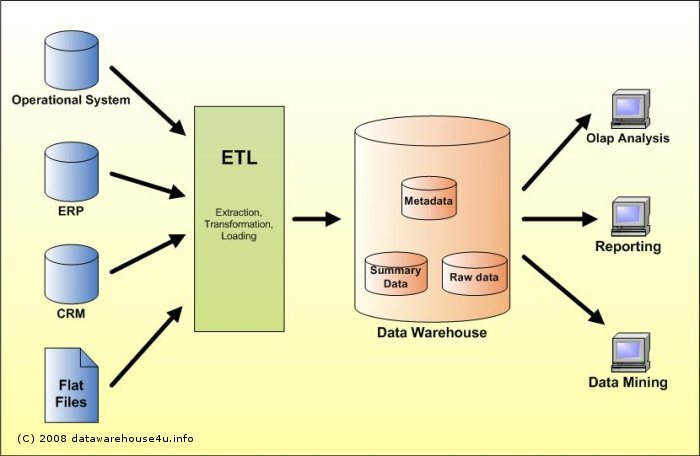
\includegraphics[width=\textwidth]{dw.jpg}
\caption{Loan Application Flow Chart}{Source: http://libertyrva.com}
\end{figure}


One can install packeges in r studio using common  install.packages(<packagename>).what is r packages, how to use r packege, which are essential. This packages is used for following purpose

\subsection{Data Extraction:} Prior building predictive model in R one, need to process and analyse the data. The primary objective is to identify any outliers and to normalise the available data set. \cite{sola1997importance}, observed that un-normalized data tends to increase square mean error and then deviate the model prediction. Therefore, it is important to treat data and normalised it's all variables so that model works with high precision and accuracy. One can also do data pre-processing using R as well, but Alteryx provides graphical user interface to select features and settings that makes whole data processing phase easy and fast\\

\textbf{Alteryx Desginer} tool allow one to build workflow to prepare data from multiple data sources on the go and by using features such as 'Select', 'Random Sample', 'Transform' and 'Output' one can easily prepare data for the predictive model \citep{dinsmore2016self}. Alteryx can process large amount of dataset and optimized it to be ready for data modelling in R.

\begin{center}
\begin{figure}[ht]
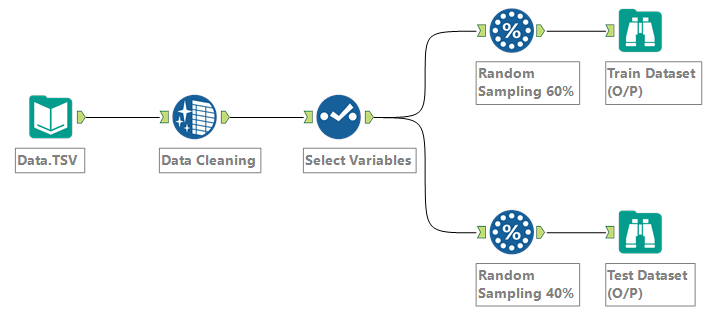
\includegraphics[width=\textwidth]{dataprocess.png}
\centering
\caption{Data Processing using Alteryx}{\textbf{Source:} Designed using in Alteryx Designer v11}
\label{fig:dataprocessing}
\end{figure}
\end{center}

In fig.\ref{fig:dataprocessing}, raw data has been read using \emph{Input tool}, then null values, white spaces etc removed using \emph{Cleansing Tool} and variables selection has been done using \emph{Select Tool}. To create train data set and test data set \emph{Random Sample \% tool}, which allows generating sample datasets.\\

\subsection{Data Transformation}
In Alteryx, there is no provision to normalize data. Processed data from Alteryx is loaded into \textbf{R Studio} for data normalization or scaling using in built functions such as scale($<variable>$) and log($<variable>$) on $LoanBalance$, $PropertyValue$, $InterestIncome$ and $AnnualPYMT$ as these variables are crucial paramters for credit scoring to make unbaised prediction model.\\

\textbf{R Studio}: Data from Alteryx is loaded to R Studio for the development of prediction model. R is used to identify patterns or correlation in variables using \emph{ggplot2}, \emph{plot.ly}, \emph{leaflets}. Two predictive models have developed based Logistic Regression and Decision Tree algorithms and both models performance evaluated concerning accuracy. Trained model is saved on the hard drive and loaded in Tableau, and with the help of R Server, Tableau allows the user to build dynamic visualizations. In Tableau, calculated fields can dynamically invokes R enginge to perform calculations and then R results output values back to Tableau, so that visualizations can be designed.\\


\subsection{Data Loading}
\textbf{Integration of R in Tableau}: Processed and transformed data is loaded into Tableau for building business dashboards. Credit analyst or auditors will use the dashboard to identify locations where the most number of loan default happenings or identify those portfolios which have provided incorrect information, etc. business decisions can be made with the help of credit scoring dashboard.\\

\textbf{Installtion of R Server:} Local instance of R Server is deployed by installing \emph{Rserve} package from R console. To invoke R Server with following command:
      \begin{verbatim}
      install.packages("Rserve")
      library(Rserve)
      Rserve()
      \end{verbatim}

\textbf{Setting in Tableau}:\\

In Tableau, go to \emph{Settings and Performance} under \emph{Help} menu and then select \emph{Manage External Service Connection}. Following settings are required to connect with R server:
      \begin{verbatim}
      Server: "localhost" or "127.0.0.1
      Port: 6311
      \end{verbatim}

R scripts are written in calculated fields of Tableau to make calls to R using in built functions in Tableau such as \emph{SCRIPT\_STR} and \emph{SCRIPT\_REAL}



\subsection{Model}

Accuracy reduced to 25\% after scaling variables. Compare difference between model performance and how it is improved.

How we implemented the model

Explaing Limitations of Algorithm and why one algo is better

\subsubsection*{Logistic Regression}

Overview:

Settings:

Output:

Limitations:

Enhancement:


\subsubsection*{Decission Tree}

Overview:

Settings:

Output:

Limitations:

Enhancement:



Intially, Logistic Regression and Decsion tree were giving accuracy of 99.31\% which is practially not possible in credit scoring. during this research work we found that various other researchers also pointed out that Logistic regression is much better modelling technique than any other statsical techqnique. For Instance Mr.x noted in work that neural network can work at par with logistic regression model provided that the target variable is predict result in yes or no.\\

Similarly decision tree has other limitations with respect to number of possible nodes and leafs for making creteria. hence decision tree end with less number of rules. Mr. Y compared the performance of Decesion tree and LR and found LR performance is higher than 5\%

As per dasssssssssssh paper 25 - 30\% error is expected in credit rating system because human nature is quite difficult to predict. Similar in this scenario it is quite complex to various parameter to consider to build solid system which have high accuracy. One of the leading bank in Ireland in past attempted to consider upto 600 parameter to all possible cases of credit using Artificial Intelligence 
testiing of model.


FUTURE SCOPE IS AI of this credit scoring

\section{Deployment \& Connection Setup}



